\documentclass[../main.tex]{subfiles}
 
\begin{document}
	\section{Magnetism}
	\begin{preamb}
		Magnets were discovered by who knows who at who knows when. All I know is we have to study them now thanks to lodestone sailor people.
	\end{preamb}
	\subsection{Magnets}
	\pdef{Magnetic Materials}{Magnetic materials are materials that can be attracted to a magnet.}
	The four materials you probably remember from primary school are: iron, nickel, cobalt, and steel.
	\pdef{Non-magnetic Materials}{Non-magnetic materials are materials that cannot be attracted to a magnet.}
	\pdef{Law of Magnetic Poles}{The law of magnetic poles states that like poles repel and unlike poles attract.}
	Some properties magnets exhibit are
	\begin{itemize}
		\item Magnets have two poles: north and south.
		\item Magnets point in the north-south direction when suspended.
		\item Like poles repel, unlike poles attract.
	\end{itemize}
	Using the property that magnets can repel, we can do the repulsion test to see if an object is a magnet or just a magnetic material.
	
	\subsection{Magnetic Induction}
	\pdef{Magnetic Induction}{Magnetic induction is the process whereby an object made of a magnetic material becomes a magnet when it is near or in contact with a magnet.}
	That means magnetic materials become magnets when in contact or near a magnet.
	
	\subsection{Magnetisation and Demagnetisation}
	\pdef{Theory of Magnetism}{\textit{(This is not in syllabus.)} A magnet is made up of many magnetic domains which are made up of atoms that have a ferromagnetic property.}
	\subsubsection{Magnetisation}
	You can make a magnet either by stroking it with another magnet, or using electricity to make an electromagnet.
	\begin{center}
		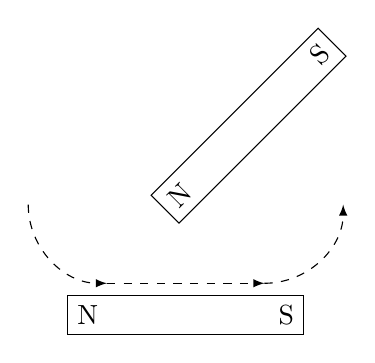
\begin{tikzpicture}
			\draw (0,0) rectangle (3,0.5);
			\node[anchor=west] at (0,0.25) {N};
			\node[anchor=east] at (3,0.25) {S};
			\draw[rotate=45] (2,0) node[anchor=south west, rotate=45] {N} rectangle (5,0.5) node[anchor=north east, rotate=45]{S};
			\draw[dashed, -latex] (0.5,0.65) -- (2.5,0.65);
			\draw[dashed, -latex] (2.5,0.65) arc (270:360:1);
			\draw[dashed, -latex] (-0.5,1.65) arc (180:270:1);
		\end{tikzpicture}
	\end{center}
	The pole that touches the magnetic object first will be the pole of that magnetic object at that point.
	
	For the electromagnet, refer to chapter 21.
	
	\subsubsection{Demagnetisation}
	To demagnetise a magnet you first have to orient it in the \textbf{east-west direction}. Then there are three ways to do this.
	\begin{enumerate}
		\item \textbf{Hammering:} Hammering a magnet placed in the east-west direction alters the alignment of the magnetic domains, causing the magnet to lose its magnetism.
		\item \textbf{Heating:} Strongly heating a magnet and letting it cool in an east-west orientation will cause the magnet to lose its magnetism. The temperature to heat the magnet up to such that the atoms lose the magnetism is called the Curie temperature.
		\item \textbf{Electrical Method:} Place a magnet in a solenoid in the east-west direction and connect an alternating current supply. Withdraw the magnet while the alternating current is flowing in the solenoid until it is some distance away.
	\end{enumerate}

	\subsection{Magnetic Fields}
	\pdef{Magnetic Field}{A magnetic field is the region surrounding a magnet, in which a body of magnetic material experiences a magnetic force.}

	Magnetic field lines \textbf{cannot cross}.
	
	Magnetic monopoles \textbf{do not exist}.
	
	Field lines point from \textbf{north poles} to \textbf{south poles.}
	\begin{center}
		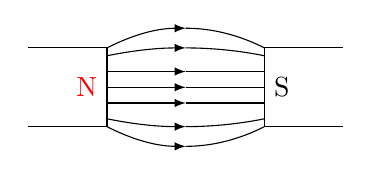
\begin{tikzpicture}
			\draw (0,0) -- (1,0) -- (1,1) node[pos=0.5, anchor=east] {\color{red} N} -- (0,1) ;
			\draw (4,0) -- (3,0) -- (3,1) node[pos=0.5, anchor=west] {S} -- (4,1);
			\draw[latex-] (2,1.25) parabola (1,1);
			\draw[latex-] (2,-0.25) parabola (1,0);
			\draw (2,1.25) parabola (3,1);
			\draw (2,-0.25) parabola (3,0);
			\draw[latex-] (2,1) parabola (1,0.9);
			\draw[latex-] (2,0) parabola (1,0.1);
			\draw (2,1) parabola (3,0.9);
			\draw (2,0) parabola (3,0.1);
			\foreach \y in {0.3,0.5,0.7} \draw[-latex] (1,\y) -- (2,\y);
			\foreach \y in {0.3,0.5,0.7} \draw (2,\y) -- (3,\y);
		\end{tikzpicture}
	\end{center}
	
	The magnetic field of a magnet can be plotted by sprinkling iron filings around it, or plotting it with a plotting compass.
	
	To use a plotting compass, align a magnet in the north-south direction first. Then using a plotting compass, from the north pole of the magnet, draw a point at where the compass points to. Then continue this and connect the lines. Remember that plotting compasses point in the direction of the field lines.
	
	For attraction and repulsion of two magnetic poles use this lovely diagram that I could not draw so I had to source it online.
	\begin{center}
		\includegraphics[width=0.85\linewidth]{graphics/magnetismFieldLines}\footnote{phys.libretexts.org}
	\end{center}

	\subsection{Temporary and Permanent Magnets}
	Magnetic materials can either be ``soft'' or ``hard''. An example of a soft magnetic material is iron. An example of a hard magnetic material is steel.
	\begin{itemize}
		\item \textbf{Magnetisation} \begin{itemize}
			\item Hard magnetic materials are difficult to magnetise and demagnetise.
			\item Soft magnetic materials are easier to magnetise and demagnetise.
		\end{itemize}
		\item \textbf{Uses} \begin{itemize}
			\item Hard magnetic materials are used to make permanent magnets.
			\item Soft magnetic materials are used to make temporary magnets.
		\end{itemize}
		\item \textbf{Interaction with Field Lines} \begin{itemize}
			\item Hard magnetic materials do not allow magnetic fields to pass through it as easily as soft magnetic materials.
			\item Soft magnetic materials allow magnetic fields to pass through it with ease.
		\end{itemize}
	\end{itemize}
\end{document}